\chapter{马氏模型和隐马氏模型}

Markov Model
Page rank算法和Markov Model
Hidden Markov Model (HMM)
HMM的理论基础
HMM的应用

\section{马氏模型}

让我们从一个简单的例子谈起。假设某大学有三个食堂A、B、C。为了估计各食堂的就餐人数,针对不同食堂就餐者设计了一项调查,
以询问其今后有多大的可能性选择不同的食堂就餐。调查显示:在食堂A就餐的人中$p_{aa}$部
分仍然回到食堂$A$,有$p_{ab}$部分选择食堂B,$p_{ac}$部分选择食堂$C$;
在食堂$B$就餐的人中$p_{bb}$部分仍然回到食堂$B$,有$p_{ba}$部分选择食堂$A$,$p_{bc}$部
分选择食堂$C$;在食堂$C$就餐的人中$p_{cc}$部分仍然回到食堂$C$,有$p_{ca}$部分选择食堂$A$,
$p_{cb}$部分选择食堂$B$。如图(\ref{MarkovModel-Cafeteria})所示。
%-------------------------------------------------------------------------------
\begin{figure}[ht]
\centering
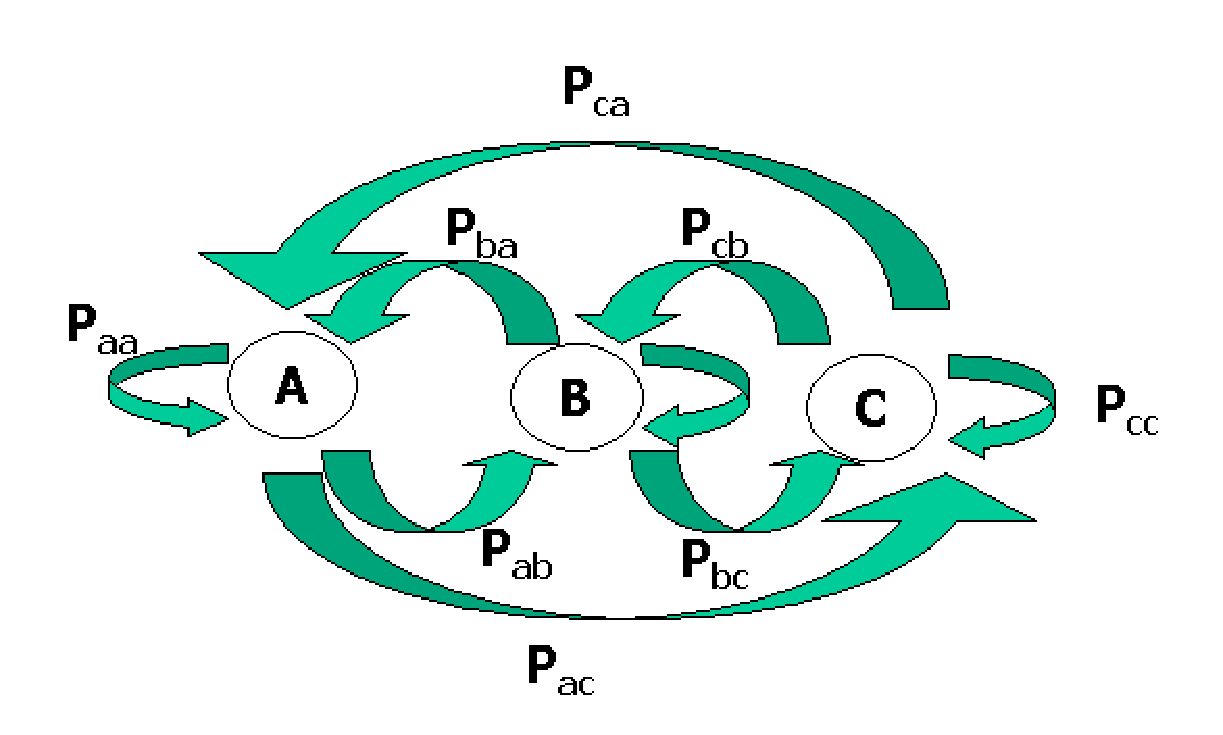
\includegraphics[width=3in]{MarkovModel-Cafeteria.eps}
\caption{食堂就餐选择意愿图} \label{Fig:MarkovModel-Cafeteria}
\end{figure}
%-------------------------------------------------------------------------------

令$A_n$, $B_n$,$C_n$分别为第$n$天在食堂$A$, $B$, $C$就餐的人数占学校总人数的比例。
假设学校只有$A,B,C$三个食堂,而且同学只能在其中之一就餐。那么
$$
\begin{aligned}
   & A_{n+1}=p_{aa}A_{n}+p_{ba}B_{n}+P_{ca}C_{n}\\
   & B_{n+1}=p_{ab}A_{n}+p_{bb}B_{n}+P_{cb}C_{n}\\
   & C_{n+1}=p_{ac}A_{n}+p_{bc}B_{n}+P_{cc}C_{n}\\
\end{aligned}
$$
矩阵表达形式如下,
$$
\begin{aligned}
& (A_{n+1}, B_{n+1}, C_{n+1})\\
=&(A_{n},B_{n},C_{n})
\left(
\begin{array}{ccc}
  p_{aa} & p_{ab} & p_{ac}\\
  p_{ba} & p_{bb} & p_{bc}\\
  p_{ca} & p_{cb} & p_{cc}\\
\end{array}
\right)\\
\end{aligned}
$$
最终的问题是:$A_n,B_n,C_n$的极限是否存在?若极限存在,则
$$
%\begin{aligned}
(x,y,z)
=(x,y,z)
\left(
\begin{array}{ccc}
  p_{aa} & p_{ab} & p_{ac}\\
  p_{ba} & p_{bb} & p_{bc}\\
  p_{ca} & p_{cb} & p_{cc}\\
\end{array}
\right)
%\end{aligned}
$$
如果用变换的角度来看,这是一个不动点问题。

若初值为$\pi_0=(A_0,B_0,C_0)$,并令$P$为上式中的矩阵,则
$$
(A_{n},B_{n},C_{n})=\pi_{0} P^{n}
$$
若$\pi=(1/3,1/3,1/3)$,$P$由下面的矩阵给出,我们可以具体计算$(A_n,B_n,C_n)$
$$
P=\left(
 \begin{array}{ccc}
   0.75 & 0.05 & 0.20\\
   0.20 & 0.60 & 0.20\\
   0.40 & 0.20 & 0.40\\
 \end{array}
\right)
$$

\begin{table}
\centering
\begin{tabular}{|cccc|cccc|}
\hline
n &  $An$ & $Bn$ & $Cn$ & n &  $An$ & $B_n$ & $C_n$\\
1  & 0.4500  0.2833 & 0.2667 & 11 & 0.5553 & 0.1947 & 0.2500\\
2  & 0.5008  0.2458 & 0.2533 & 12 & 0.5554 & 0.1946 & 0.2500\\
3  & 0.5261  0.2232 & 0.2507 & 13 & 0.5555 & 0.1945 & 0.2500\\
4  & 0.5395  0.2104 & 0.2501 & 14 & 0.5555 & 0.1945 & 0.2500\\
5  & 0.5468  0.2032 & 0.2500 & 15 & 0.5555 & 0.1945 & 0.2500\\
6  & 0.5507  0.1993 & 0.2500 & 16 & 0.5555 & 0.1945 & 0.2500\\
7  & 0.5529  0.1971 & 0.2500 & 17 & 0.5555 & 0.1945 & 0.2500\\
8  & 0.5541  0.1959 & 0.2500 & 18 & 0.5555 & 0.1945 & 0.2500\\
9  & 0.5548  0.1952 & 0.2500 & 19 & 0.5555 & 0.1945 & 0.2500\\
10 & 0.5551  0.1949 & 0.2500 & 20 & 0.5555 & 0.1945 & 0.2500\\
\hline
\end{tabular}
\end{table}

%-------------------------------------------------------------------------------
\begin{figure}[ht]
\centering
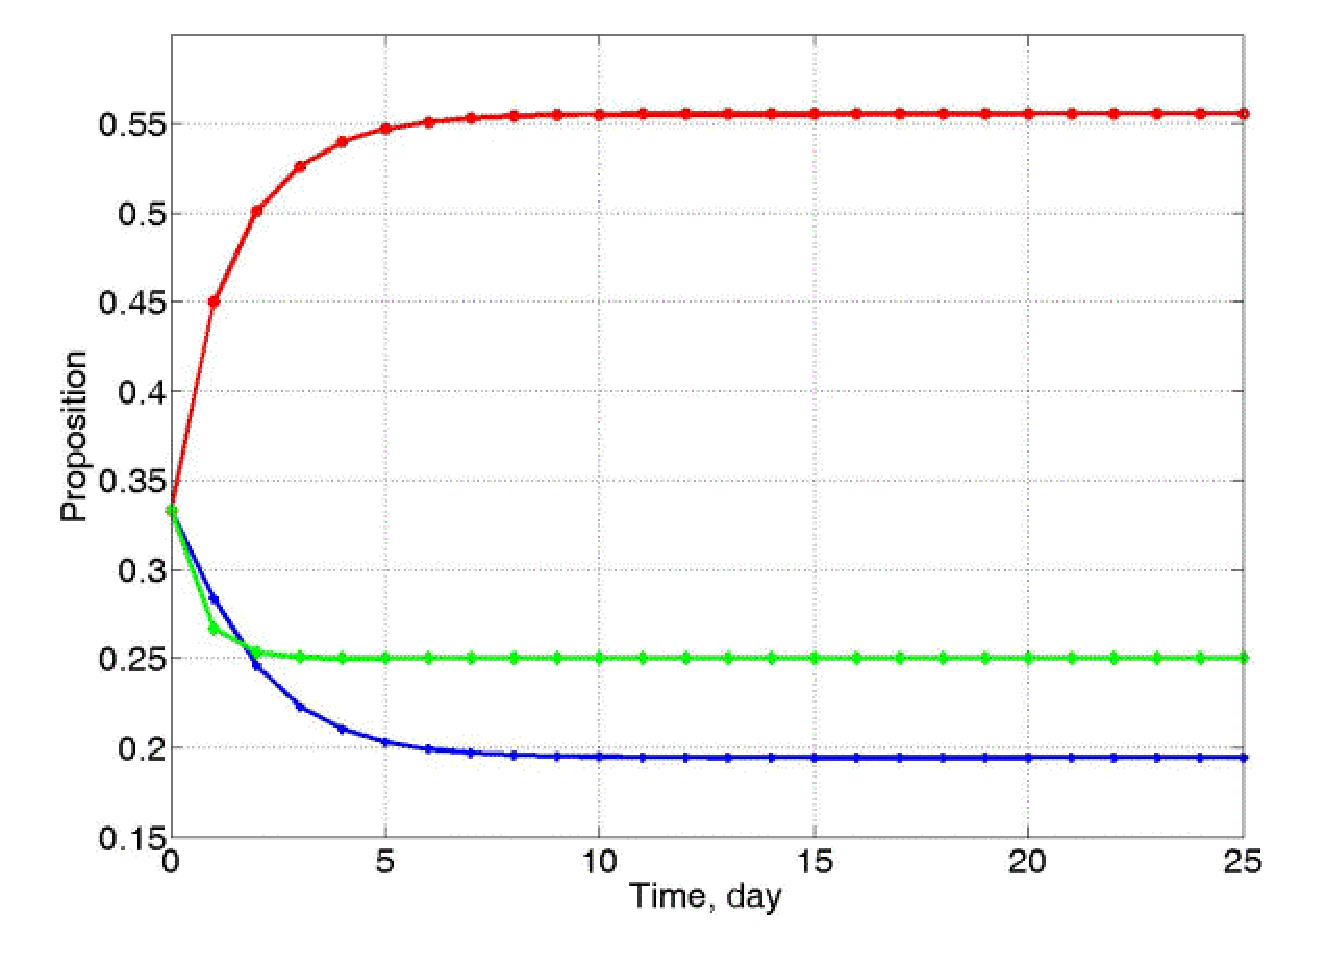
\includegraphics[width=3in]{DynamicsNumber.eps}
\caption{$(A_n,B_n,C_n$动态演化图} \label{Fig:DynamicsNumber}
\end{figure}
%-------------------------------------------------------------------------------
可以看出,从第十四步开始,在千分之一的精度下系统收敛到$(0.5555,0.1945,0.2500)$,而且收敛的
基本上是以指数速度收敛。类似于上面的计算,对于上面的例子我们还可以换一个起点进行迭代,可以
看到收敛现象依然存在,而且收敛的结果与起点无关(具体计算不再显示)。
出现这样的现象一点都不奇怪,后面将会看到它有严格的理论保证。


分析刚才的例子,有其特殊性。其一,每一步活动只与当前处在什么“状态”有关,
与过去的“状态”没有关系(无后效性)。其次矩阵$P$也有其特殊性:每行和为1,表示下一个时刻的状态必须在A、B、C中之一。

马尔可夫链模型,简称马氏链。

\section{PageRank算法和马氏模型}


\section{隐马氏模型}

隐马氏模型是一个统计模型,其经典理论由L.E.Baum等在六十年代末七十年代初所给出。
随后这一模型于七十年代中期由Jenik等应用到语音识别领域中来,逐步发展成为语音识
别中最为瞩目、最有效的技术之一。随后,这一模型也被大量应用于文字识别之中。九
十年代,随着人类基因组计划的启动,推动了各种计算机技术在生物学科中的应用,产生
了“计算生物学”这门交叉学科,隐马氏模型就是其中最为广泛应用的数学模型之一,
其在基因识别,基因表达数据处理等方面都有非常成功的应用,比如目前最有效的基因识别
软件GenScan的核心技术就是基于隐马氏模型的。


在介绍隐马氏模型之前,让我们先看一个例子。

例一(韦小宝的骰子):金庸武侠小说$\langle\!\langle$鹿鼎记$\rangle\!\rangle$很多人都爱看,
对书中主人公韦小宝更是非常熟悉。
韦小宝嗜赌成性,基本上是逢赌必赢。他的秘密武器是出千——用他那灌了铅的骰子。现在用$A$表示使用
正常的骰子,$B$表示使用灌铅的骰子。假设用灌铅骰子有很大的概率出高点(5和6),出5和6的概率为$0.3$,
出其它点的概率是$0.1$。使用正常骰子出每个点的概率都一样为$\frac{1}{6}$。假设韦小宝在选择是否用他那
灌铅的骰子服从马氏链(由前面的讨论知道,只有确定了初概率和转移概率后,马氏链被确定下来),开始时
刻以$0.4$的概率使用灌铅的骰子,其它时刻的选择依赖于前一个时刻的选择。具体来说,如果当前处在A,下一时
刻还是A的概率是$0.8$,是B的概率是$0.2$;如果当前处在$B$,下一时
刻还是B的概率是$0.9$,是A的概率是$0.1$。如图(\ref{Fig:DiceTransitionProbability})所示。
%-------------------------------------------------------------------------------
\begin{figure}[ht]
\centering
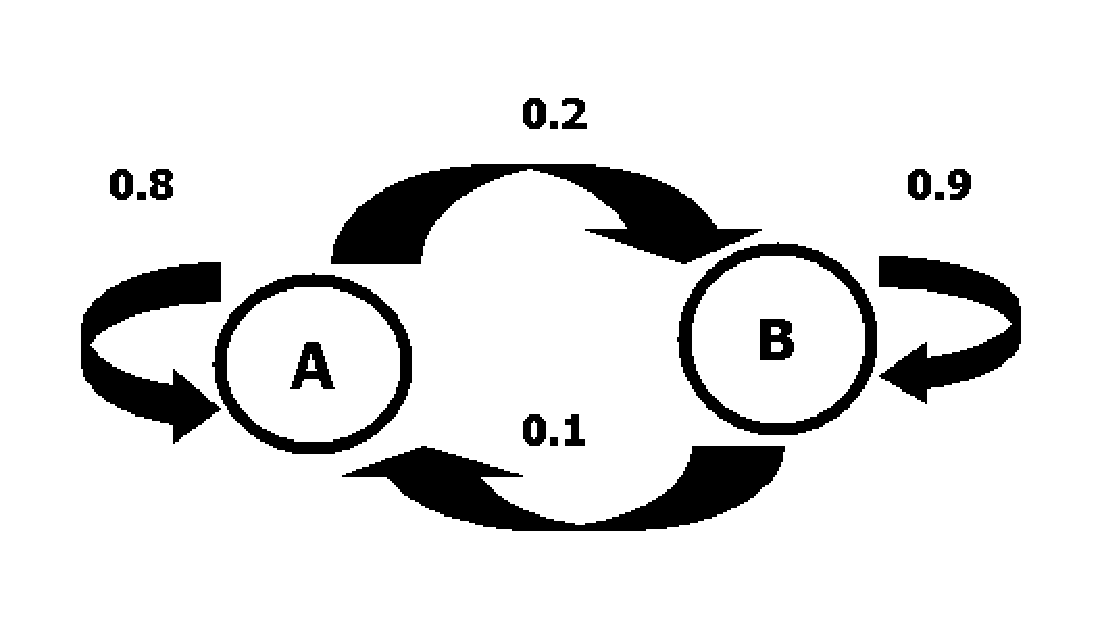
\includegraphics[width=3in]{DiceTransitionProbability.eps}
\caption{掷骰子中的转移概率}
\label{Fig:DiceTransitionProbability}
\end{figure}
%-------------------------------------------------------------------------------
如果他掷出了这样一串点数
$$
O=\{1,3,4,5,5,6,6,3,2,6)\}
$$
你能猜出他在什么时候出千了吗?


在以上例子中含有两个随机过程,一个是可以直接观测到的
观察过程,另一个是不能直接观测到的马氏过程(隐过程)。隐过程与观测过程由一定
的概率相关联。他们就是隐马氏模型。下面给出隐马氏模型的定义。

定义: 隐马氏链模型 (HMM)包括一个状态马氏链
 $X=\{x_{t},T\geq t \geq 1\}$ 和一个由状态过程所决定的观测随机过程
 $Y=\{y_{t}:T\geq t\geq 1\}$,其中状态马氏链 $X$ 不可观测,它只能由观测随机
过程来间接地了解。

需要说明的是,状态过程的马氏性可以是多步的,也可以是单步的,这完全由实际问题
所决定,一般的情况是,多步马氏性需要更多的参数来描述,相应地模型也具有
更大的灵活性;观测过程和状态过程是相关的,这种相关性用概率的语言来描述就是,对
于$\forall n$,条件概率
$$
\mbox{Pr}(y_{n})=V_{k_{n}} | x_{n}=S_{i_{n}}, \cdots, x_{0}
      =S_{i_{0}}, y_{n-1}=V_{k_{n-1}}, \cdots, y_{1}=V_{k_{1}})
$$
是已知的,对具体的问题往往需要有不同复杂程度的相互关系要求。最简单的情形为:
$$
\begin{aligned}
&\mbox{Pr}(y_{n}=V_{k_{n}} | x_{n}=S_{i_{n}}, \cdots, x_{0}=S_{i_{0}}, y_{n-1}=V_{k_{n-1}}, \cdots, y_{1}=V_{k_{1}})\\
&=\mbox{Pr}(y_{n}=V_{k_{n}} | x_{n}=S_{i_{n}})\\
&=\cdots\\
&=\mbox{Pr}(y_{1}=V_{k_{1}} | x_{1}=S_{i_{1}})\\
\end{aligned}
$$
如果同时状态过程是单步马氏的,可用下表来说明两个过程之间的关系
\begin{table}
 \centering
   \begin{tabular}{|c|c|c|c|c|c|}
     \hline
       t & 1 & 2 & 3 & $\cdots\cdots$ & T \\
      \hline
        观察量 $y_{t}$ & $y_{1}$ & $y_{2}$ & $y_{3}$
                       & $\cdots\cdots$ & $y_{T}$ \\
      \hline
        隐状态 $x_{t}$ & $x_{1}$ & $x_{2}$ & $x_{3}$
                      & $\cdots\cdots$ & $x_{T}$ \\
      \hline
        两者联系 & P$(y_{1}| x_{1})$ &P$(y_{2}| x_{2})$ & P$(y_{3}| x_{3})$
              & $\cdots\cdots$ & P$(y_{T}| x_{T})$\\
      \hline
   \end{tabular}
   \caption{HMM定义说明}
\end{table}

从上表可以看出,要描述一个 HMM 所需的参数集为:
\begin{enumerate}
   \item[1.]   系统结构与参数 \\
        (1)   状态集合 \quad ${\cal S}=\{S_{1},S_{2}, \cdots, S_{N} \}$; \\
        (2)   观测过程状态集合 \quad ${\cal V}=\{V_{1},\cdots,V_{M}\}$,对于连续型的观测量,这个集合可以无限; \\
        (3)    观测时间指标集 \quad $\{1,2,\cdots,T\}$。 \\
   \item[2.]   概率参数 \quad $\lambda=(\pi,A,B)$,其中 \\
        (1)   初始概率 \quad $\pi=\{ \pi_{i}| \pi_{i}=\mbox{Pr}(x_{0}=S_{i})\}$; \\
        (2)   转移概率 \quad $A=\{ (a_{ij})_{N\times N}| a_{ij}=\mbox{Pr}(x_{t}=S_{j}|x_{t-1}=S_{i}) \}$; \\
        (3)   观测特征的条件分布 \quad $B=\{ (b_{j}(k))_{N \times M} |  b_{j}(k)=\mbox{Pr}(y_{t}=V_{k}|x_{t}=S_{j} \}$。
\end{enumerate}
因此,要描述这样一个隐马氏模型需要的参数个数是
$$
(N-1)+N\times (N-1)+ N \times (M-1)=N \times (N+M-1)-1
$$

HMM广泛地应用于模式识别问题之中,一般对每个模式建立一个HMM
参数模型,而要识别一个样本就是给出该样本的观测过程$y=(y_{1},y_{2},\cdots,y_{T})$,
找出此样本出自那一个模型$\lambda^{\ast}$,这就是所谓的识别问题,如例二所示;另一方面,
给定模型参数和某个观测序列,需要了解其背后的隐状态序列,这就是所谓的解码问题,如例一所示;
最后就是参数的估计问题。在前面的韦小宝的骰子的例子中,我们是直接给出了韦小宝掷骰子的规律,这个
规律怎么得到呢,只可能从他大量的实战记录中估计出来,这实际是一个归纳学习的问题,故称之为学习
问题。所幸的是,对于隐马氏问题,这三个问题-识别问题、解码问题和学习问题都有很完整的理论和算
法来回答,构成了隐马氏模型理论。以下逐一介绍隐马氏模型理论。

\section{隐马氏模型理论和算法}

隐马氏链理论包括包括概率计算的前向、后向算法,隐状态确定的Viterbi 算法
和参数估计的Baum\_Welch公式。分别对应于前面提到的识别问题、解码问题和学习问题。

\subsection{识别问题}
给定一个观察量序列 $y=(y_{1}y_{2}\cdots
y_{T})$,一个首要的问题是计算 其在某个模型 $\lambda=(\pi,A,B)$
下的概率 $\mbox{Pr}(y |\lambda)$,以
这个概率来衡量其在不同模型下的相似度,然后按照 Bayes 统计原则,取
 $
   \lambda^{\ast}=\mathop{\mbox{Argmax}}\limits_{i}
                 \{\mbox{Pr}( y| \lambda_{i}) | \lambda \mbox{取遍一切可能的模式}\}
$ 为识别结果 --- 认为样本 $y$ 出自模式
$\lambda^{\ast}$,因为这个模式的可能性最大。

 设 $x=(x_{1},\cdots,x_{T}),y=(y_{1},\cdots,y_{T})$,按隐马氏模型的定义,易知
 $$
\begin{aligned}
 &\mbox{Pr}(X=x | \lambda)=\pi_{x_{0}}a_{x_{0}x_{1}}\cdots a_{x_{T-1}x_{T}}\\
 &\mbox{Pr}(Y=y | X=x,\lambda)=b_{x_{1}}(y_{1})\cdots b_{x_{T}}(y_{T})\\
 &\mbox{Pr}(Y=y |\lambda)=\sum\limits_{X=x}\mbox{Pr}(Y=y |X=x,\lambda)
            \mbox{Pr}(X=x | \lambda)\\
 &=\sum\limits_{x=(x_{1},x_{2},\cdots,x_{T})}
   \pi(x_{1})b_{x_{1}}(y_{1})
   a_{x_{1}x_{2}}b_{x_{2}}(y_{2})\cdots
   a_{x_{T-1}x_{T}}b_{x_{T}}(y_{T})\\
\end{aligned}
$$
上面的公式中要对状态的所有可能位形求和,因而是指数级复杂度的
(其计算量为 $2TN^{T}$), 当 $N$
较大时如此大的计算量几乎无法实现。前向算法和后向算法给出了计算
$\mbox{Pr}(Y = y |\lambda)$  的多项式级复杂度的计算方法。

令 $\alpha_{t}(i)=\mbox{Pr}(y_{1},y_{2},\cdots,y_{t},x_{t}=i |
\lambda)$
$$
\begin{aligned}
 \alpha_{t+1}(i)=&\mbox{Pr}(y_{1},y_{2},\cdots,y_{t+1},x_{t+1}=i | \lambda)\\
          =&\sum\limits_{j}\mbox{Pr}(y_{1},y_{2},\cdots,y_{t+1},
   x_{t}=j,x_{t+1}=i | \lambda)\\
      =&\sum\limits_{j}\alpha_{t}(j)a_{ji}b_{i}(y_{t+1})\\
\end{aligned}
$$
因此有如下前向算法 (Forward algorithm)。

\vspace*{\baselineskip} \noindent {\songti\zihao{5} 前向算法(Forward
algorithm)}
\begin{enumerate}
   \item  初始化: $\alpha_{1}(i)=\pi_{i}b_{i}(O_{1})$,\quad $i=1,2,\cdots,N$;\\
   \item  迭代: $\alpha_{t+1}(i)=(\sum\limits_{j=1}^{N}\alpha_{t}(j)a_{ji})b_{i}(O_{t+1})$,\\
                  \quad $1\leq i\leq N$,$t=1,\cdots,T-1$;\\
   \item   结果: $\mbox{Pr}(O |\lambda)=\sum\limits_{i=1}^{N}\alpha_{T}(i)$.
\end{enumerate}
 同理令 $\beta_{t}(i)=\mbox{Pr}(y_{t+1},y_{t+2},\cdots,y_{T} |x_{t}=i,\lambda)$
$$
\begin{aligned}
\beta_{t}(i)=&\sum\limits_{j}\mbox{Pr}(y_{t+1},y_{t+2},\cdots,y_{T},
   x_{t+1}=j |x_{t}=i,\lambda)\\
          =&\sum\limits_{j}\beta_{t+1}(j)a_{ij}b_{j}(y_{t+1})\\
\end{aligned}
$$
有如下的后向算法 (Backward algorithm)。

\vspace*{\baselineskip} \noindent {\songti\zihao{5}
后向算法(Backward algorithm)}
\begin{enumerate}
   \item  初始化: $\beta_{T}(i)=1$,\quad $1\leq i \leq N$;\\
   \item  迭代: $\beta_{t}(i)=\sum\limits_{j=1}^{N}\beta_{t+1}(j)a_{ij}b_{j}(O_{t+1})$,
                  \quad $1\leq i\leq N$,$t=T-1,\cdots,1$;\\
   \item   结果: $\mbox{Pr}(O |\lambda)=\sum\limits_{i=1}^{N}\beta_{1}(i)b_{i}(O_{1})$.\\
\end{enumerate}
 这两种算法的计算量为 $T\times N^2$  阶的。

\subsection{译码问题}
给定观察量序列 $Y=(y_{1}y_{2}\cdots
y_{T})$,我们往往需要知道观测链所对应的隐状态
序列$\hat{X}=(\hat{x_{1}}, \hat{x_2},\cdots,\hat{x_T})$是什么。根据不同的优化原
则,我们可以得到不同的状态序列。
 \begin{enumerate}
 \item[1.]  原则 1:  单点的状态最优。即在每一个时刻,求最可能的状态
 $$
\begin{aligned}
 & \gamma_{t}(i)=Pr(X_{t}=i | Y)\\
 & \hat{x_{t}}=\mathop{\mbox{Argmax}}\limits_{i} \gamma_{t}(i)
\end{aligned}
$$
其中$\gamma_{t}(i)$可以计算,
$$
  \begin{aligned}
    & \gamma_{t}(i)=Pr(X_{t}=i | y_{1},y_{2},\cdots, y_{T},\lambda)\\
        &=\frac{Pr(X_{t}=i, y_{1},\cdots, y_{T} | \lambda)}{Pr(y_{1},\cdots, y_{T}| \lambda)}\\
        &=\frac{Pr(X_{t}=i, y_{1},y_{2},\cdots, y_{T}| \lambda)}{\sum\limits_{i}Pr(X_{t}=i, y_{1},y_{2},\cdots, y_{T} | \lambda)}\\
        &=\frac{Pr(y_{t+1},\cdots, y_{T} | x_{t}=i,y_{1},\cdots,y_{t},\lambda)Pr(x_{t}=i,y_{1},\cdots,y_{t} | \lambda)}{\sum\limits_{i}Pr(X_{t}=i, y_{1},y_{2},\cdots, y_{T} | \lambda)}\\
        &=\frac{\alpha_{t}(i)\beta_{t}(i)}{\sum\limits_{i}\alpha_{t}(i)\beta_{t}(i)}
  \end{aligned}
$$
即完全由前向概率和后向概率给出。

 \item[2.]   原则2:路径最优。前者是每一个时刻分别确定状态,没有考虑
到前后两个状态之间的制约关系,因此完全有可能得到的状态序列是不存在
的。基于这种原因,考虑路径最优的原则就是很自然的了。即选取状态序列
$\hat{X}=(\hat{x_{1}}, \hat{x_2},\cdots,\hat{x_T})$,使得
$$
\begin{aligned}
  & Pr(\hat{x_{1}}, \hat{x_2},\cdots,\hat{x_T} | y_{1},\cdots,y_{T})\\
  & \geq Pr ( x_{1},x_{2},\cdots,x_{T} | y_{1},\cdots,y_{T})\\
\end{aligned}
$$
由Bayesian公式有
$$
\begin{aligned}
  & Pr((x_1, x_2,\cdots,x_T | y_{1},\cdots,y_{T})\\
  & =\frac{Pr( x_1, x_2,\cdots,x_T, y_1,\cdots,y_T)}
      {Pr(y_{1},\cdots,y_{T})}
\end{aligned}
$$
又由于序列 $Y$ 给定, 因此问题等价于找最优状态序列X使联合
概率$Pr(x_1,x_2,\cdots,x_T;y_1,y_2,\cdots,y_T)$最大。
这是一个多步决策问题,更重要的是模型具有马氏性,那么对应于这个
多步决策问题具有”无后效性“,因此可以借助于动态规划的思想,化整为零,
通过递推方式求解。相应的递推变量可以如下定义,
$$
     \delta_{t}(i)=\max\limits_{x_{1}\cdots,x_{t-1}}
        \mbox{Pr}(x_{1}\cdots,x_{t-1},x_{t}=i,
  y_{1}\cdots y_{t}|\lambda)
   $$
则
 $$
\begin{aligned}
    \delta_{t+1}(i)=&\max\limits_{x_{1}\cdots,x_{t-1},x_{t} }
        \mbox{Pr}(x_{1}\cdots,x_{t-1},x_{t},x_{t+1}=i,
  Y_{1}\cdots y_{t}, y_{t+1}|\lambda)\\
      =&[\max\limits_{j}\delta_{t}(j) a_{ji}] b_{i}(y_{t+1})\\
\end{aligned}
$$

这种选择最优状态序列的过程就是著名的 Viterbi 算法。为方便起见,对任意状态
$i$,以$\psi_{t}(i)$记录$t$时刻时使$\delta_{t}(j)a_{ji}$最大的状态$j$。
\end{enumerate}

\vspace*{\baselineskip}
{\it
\noindent {\songti\zihao{5} Viterbi算法}
\begin{enumerate}
  \item   初始化:
 $$
    \begin{aligned}
             \delta_{1}(i)&=\pi_{i}b_{i}(O_{1})\  1\leq i\leq N \\
      \psi_{1}(i)&=0\\
    \end{aligned}
 $$
 \item   迭代,对 $t=2,3,\cdots,T-1;\ j=1,2,\cdots,N$,计算
 $$
    \begin{aligned}
    \delta_{t}(j)&=\max\limits_{1\leq i\leq N}[\delta_{t-1}(i)a_{ij}] b_{j}(O_{t})\\
       \psi_{t}(j)&=\mathop{\mbox{Argmax}}\limits_{1\leq i\leq N}[\delta_{t-1}(i)a_{ij}]\\
    \end{aligned}
 $$
  \item  终止:
 $$
    \begin{aligned}
       P^{\ast}&=\max\limits_{1\leq i\leq N}(\delta_{T}(i))\\
       x_{T}^{\ast}&=\mathop{\mbox{Argmax}}\limits_{1\leq i\leq N}(\delta_{T}(i))\\
    \end{aligned}
$$
\item  后推
 $$
           x_{t}^{\ast}=\psi_{t+1}(x_{t+1}^{\ast}) \qquad\qquad  t=T-1,t-2,\cdots,1
$$
\end{enumerate}
}
注记:在许多应用中,常以 $P^{\ast}$  作为 $\mbox{Pr}(O | \lambda)$的近似值。

现在可以回答例子”韦小宝的骰子“所提出的问题-什么时间出千的问题
该隐马氏模型有2个状态$A$和$B$,$6$种观测$(V_{1},V_{2},\cdots, V_{6})$,
各参数设置如下表
\begin{table}
 \centering
   \begin{tabular}{|c|c|c|}
     \hline
     &目标$A$ & 目标 $B$\\
      \hline
         $A$ & 0.8 & 0.2\\
      \hline
         $B$ & 0.1 & 0.9 \\
      \hline
         初概率 & 0.6 & 0.4\\
      \hline
   \end{tabular}
\caption{HMM参数(转移概率与初概率)}
\end{table}

\begin{table}
\centering
   \begin{tabular}{|c|c|c|c|c|c|c|}
     \hline
     & $V_1$ & $V_2$ & $V_3$ & $V_4$ & $V_5$ & $V_6$\\
      \hline
         $A $ & $\frac{1}{6}$ & $\frac{1}{6}$ & $\frac{1}{6}$ & $\frac{1}{6}$ & $\frac{1}{6}$ & $\frac{1}{6}$\\
      \hline
         $B$ & 0.1 & 0.1  & 0.1 & 0.1 & 0.3 & 0.3\\
      \hline
   \end{tabular}
\caption{HMM参数(观测特征条件分布)}
\end{table}

观测序列$Y=(1, 3, 4, 5,5 , 6, 6,3,2,6)$,用Viterbi算法
给出相应的隐状态序列$X$。
\begin{table}
\centering
\begin{tabular}{|ll||ll||ll|}
\hline
   & $y_t$  & $\delta_t(A)$ & $\Psi_t(A)$ &  $\delta_t(B)$ & $ \Psi_t(B)$\\
\hline
t=1 & 1 &   1.000x10-1 &  - & 4.000x10-2 & -\\
t=2 & 3 &   1.333x10-2 &  A & 3.600x10-3 & B\\
t=3 & 4 &   1.778x10-3 & A & 3.240x10-4 & B\\
t=4 & 5 &   3.370x10-4 & A & 1.067x10-4 & A\\
t=5 & 5 &   3.161x10-4 & A & 2.880x10-5 & B\\
t=6 & 6  &  4.214x10-6 & A & 7.776x10-6 & B\\
t=7 & 6 &   5.619x10-7 & A & 2.100x10-6 & B\\
t=8 & 3  &  7.492x10-8 & A & 1.890x10-7 & B\\
t=9 & 2 &   9.989x10-9 & A & 1.701x10-8 & B\\
t=10  &   6 &   1.322x10-9 & A & 4.592x10-9 & B\\
\hline
\end{tabular}
\caption{Viterbi算法数据演示}
\end{table}
最后得出状态序列 为$X=(AAABBBBBBB)$, 如图(\ref{Fig:ViterbiPath})所示.
%-----------------------------------------------------------------------------------------------------------------
\begin{figure}[ht]
\centering
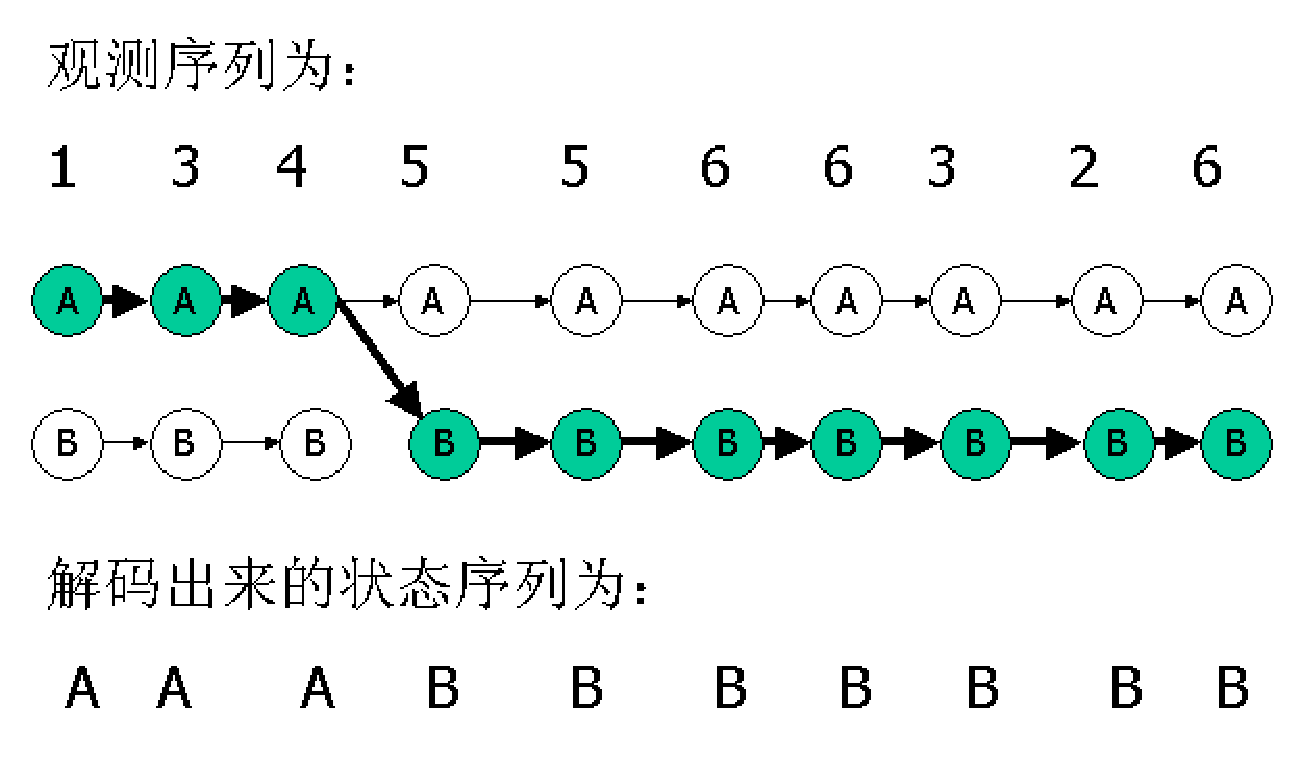
\includegraphics[width=4in]{ViterbiPath.eps}
\caption[]{Viterbi算法实例. 其中箭头表示$\psi_{t}(i)$值, 粗线表示最优路径.}
\label{Fig:ViterbiPath}
\end{figure}
%-----------------------------------------------------------------------------------------------------------------

\subsection{学习问题}
学习的目的是通过对学习样本集的统计计算,调整模型的参数,对每一个模式找到一组
最适合样本集的参数。在极大似然意义下,即为单一观测量的
 $$
\lambda^{\ast}=\mathop{\mbox{Argmax}}\limits_{\lambda}\mbox{Pr}(y
|\lambda)
$$
或多观测量的
$$
  \lambda^{\ast}
  =\mathop{\mbox{Argmax}}\limits_{\lambda}\mbox{Pr}(y^{1},\cdots,y^{K} |\lambda),
    \ K\geq 2\mbox{为常数}
$$
这里,由于参数 $\lambda$ 与隐马氏链的状态 $x$
都是未知的,要从前面的关系 式 (1.2) 得到 $\mbox{Pr}(y |\lambda)$ 或
$\mbox{Pr}(y^1, \cdots, y^{K} | \lambda)$
 的优化很困难。一种解决问题的方法是借助于模型参数和模型状态之间的交叉验证,轮番优
化参数 $\lambda$ 和隐状态,即先给定某个初始参数
$\lambda_{0}$,估计出对这组参数的最
可能状态;再在当前的状态下重新估计参数
$\lambda$,又在新的参数下重估计模型的状态
$\cdots\cdots$,如此循环直至某个收敛条件满足为止。 Baum\_Welch  算法
(或 EM 算法) 就是对这一
问题的两种比较简单易行的逐次逼近算法,即先粗略地给出某一初始参数
$\lambda_{0}$,
再由样本逐次对参数修正,使之逐次逼近真实参数。为简单起见,我们只研究
单一观测量参数估计问题,即考虑读入一个观测样本,如何修正模型参数的问题。

设模型的初步参数集合 $\lambda=\{ \pi, A, B
\}$,且读入样本的观测序列为 $y=\{ y_{1}, \cdots, y_{T} \}$,若令
$$
\begin{aligned}
  &\zeta_{t}(i,j)=\mbox{Pr}(x_{t}=i,x_{t+1}=j | y,\lambda)
    =\frac{\alpha_{t}(i)a_{ij} b_{j}(y_{t+1})\beta_{t+1}(j)}
    {\sum\limits_{i=1}^{N}\alpha_{t}(i)\beta_{t}(i)}\\
  &\gamma_{t}(i)=\mbox{Pr}(x_{t}=i | y,\lambda)
   =\frac{\alpha_{t}(i)\beta_{t}(i)}
   {\sum\limits_{i=1}^{N}\alpha_{t}(i)\beta_{t}(i)}\\
\end{aligned}
$$
其中$\alpha_{t}(i),
\beta_{t}(i)$分别为前向概率和后向概率,按照概率意义,
$\zeta_{t}(i,j)$ 表示在 $t$  时刻发生状态转移 ($i \rightarrow j$)
的频率。 相应地,$\gamma_{t}(i)=\mbox{Pr}(x_{t}=i |
y,\lambda)=\sum\limits_{j=1}^{N}\zeta_{t}(i,j)$ 为 $t$ 时刻状态为
$i$  的频率。
 $\sum\limits_{t=1}^{T-1}\gamma_{t}(i)$
为整个观察序列中状态转移从状态 $i$  出发的频率。
$\sum\limits_{t=1}^{T-1}\zeta_{t}(i,j)$ 为整个观察序列中发生状态转移
($i \rightarrow j$)  的频率。
由极大似然原则,可以想见模型参数重估计公式为
 $$
  \left\{
  \begin{array}{ll}
     \overline{\pi}_{i}&\approx(t=1)\mbox{时状态为}i\mbox{的频率}\\
     \overline{a}_{ij}&\approx\frac{\mbox{状态转移}i\rightarrow j\mbox{的频率}}
          {\mbox{状态转移从}i\mbox{出发的频率}}\\
   \overline{b}_{j}(k)&\approx\frac
           {\mbox{状态为}i\mbox{且观察量为}V_{k}\mbox{的频率}}
            {\mbox{处于状态}j\mbox{的频率}}
        \end{array}
  \right.
$$
用前向概率和后向概率表示即为
$$
\left\{
 \begin{array}{ll}
   \overline{\pi}& =\frac{\mbox{Pr}(y,x_{1}=i | \lambda)}
               {\mbox{Pr}(y | \lambda)}
       =\gamma_{1}(i)\\
   \overline{a}_{ij}
       &=\frac{\sum\limits_{t=1}^{T-1}
          \mbox{Pr}(y,x_{t}=i,x_{t+1}=j | \lambda)}
          {\sum\limits_{t=1}^{T-1}
           \mbox{Pr}(y,x_{t}=i | \lambda)}
          =\frac{\sum\limits_{t=1}^{T-1}\zeta_{t}(i,j)}
          {\sum\limits_{t=1}^{T-1}\gamma_{t}(i)}\\
     \overline{b}_{j}(k)
       &=\frac{\sum\limits_{t=1}^{T}
        \mbox{Pr}(y,x_{t}=i | \lambda) \delta(y_{t},V_{k})}
         {\sum\limits_{t=1}^{T}\mbox{Pr}(y,x_{t}=i | \lambda)}
         =\frac{\sum\limits_{t=1,y_{t}=V_{k}}^{T} \gamma_{t}(j)}
        {\sum\limits_{t=1}^{T}\gamma_{t}(j)}
  \end{array}
\right.
$$

以上我们纯粹从概率意义上给出了模型参数的重估计公式,该公式可以严格推导。在此之前,让
我们来看看其物理意义。从识别问题的分析我们知道,条件概率$\mbox{Pr}(y
| \lambda)$
可以理解为样本与参数模型的相似度,而其负对数可以理解为样本与参数模型的某种距离(Bayes距离);
那么在已知样本下,应该选择与样本最“接近”的参数集作为模型的参数。对于一个概率分布
来说,以这个距离的均值作为衡量是最合适不过的了,它就是信息论中的熵。下面我们将会
看到,参数重估计实际上就是对一个类似于相对熵的量的优化过程,而优化策略是标准的梯度算法。
为此我们先引进熵和相对熵的概念。

熵: 给定概率分布$p=\{p(x): x \in {\cal X}
\}$,则分布$p$的熵定义为
$$
    H(p)=-\sum\limits_{x \in {\cal X}} p(x) \log p(x)=E_{p}[ -log p(X)]
$$

某个概率分布的熵是具有该分布的随机变量的信息含量或者不确定度的衡量,比如说,购买彩票
的中奖率很低,那么购买彩票不中奖是可以想见的事,因而熵也小;但在抛硬币试验中我们很难
预见某一次是出正面还是反面,不确定性大,因而熵也大。

相对熵: 给定${\cal X}$的两个概率分布$p=\{p(x)\}, q=\{
q(x) \} $,则它们的相对熵定义为
$$
D(p,q)=\sum\limits_{x \in {\cal X}} p(x) \log
\frac{p(x)}{q(x)}=E_{p}[log \frac{p(x)}{q(x)}]
$$

\noindent 注:容易验证$D(p,q) \geq
0$,当且仅当$p=q$时取等号。因而文献上也称$D(p,q)$为两个概率分
布的Kullback-Leibler距离。

令
$$
   Q(\lambda^{\prime},\lambda)
=\sum\limits_{x} P(x,y | \lambda^{\prime}) \log \mbox{Pr}(x,y |
\lambda)
$$
容易验证
$$
   \begin{aligned}
  &Q(\lambda^{\prime},\lambda) - Q(\lambda^{\prime},\lambda^{\prime})\\
 =&\sum\limits_{x} \mbox{Pr}(x,y | \lambda^{\prime}) \log
    \frac{\mbox{Pr}(x,y | \lambda )}{\mbox{Pr}(x,y | \lambda^{\prime})}\\
     \leq & \sum\limits_{x} \mbox{Pr}(x,y | \lambda^{\prime})
       (\frac{\mbox{Pr}(x,y | \lambda) }{\mbox{Pr}(x,y | \lambda^{\prime})}-1)\\
 =&\mbox{Pr}(y | \lambda)- \mbox{Pr}(y | \lambda^{\prime})\\
\end{aligned}
$$

因此,由$Q(\lambda^{\prime},\lambda) \geq
Q(\lambda^{\prime},\lambda^{\prime})$, 可以得到则 $\mbox{Pr}(y |
\lambda) \geq \mbox{Pr}(y | \lambda^{\prime})$。以上事实说
明,如果给定参数$\lambda^{\prime}$,找出使$Q(\lambda^{\prime},\lambda)>Q(\lambda^{\prime},\lambda^{\prime})$
的参数$\lambda$,就有$\mbox{Pr}(y | \lambda)>\mbox{Pr}(y
|\lambda^{\prime})$,即找到了更加符合样本的
参数。从而将对$\mbox{Pr}(y |
\lambda)$的优化问题转化为对$Q(\lambda^{\prime},\lambda)$关于
$\lambda$的约束优化问题。

对于隐马氏链模型,
$$
\begin{aligned}
& \mbox{Pr}(x,y | \lambda)=\pi_{x_{0}} \prod\limits_{t=1}^{T} a_{x_{t-1} x_{t}} b_{x_{t}}(y_{t})\\
& \log \mbox{Pr}(x,y | \lambda)=\log \pi_{x_{0}} \sum\limits_{t=1}^{T} \log a_{x_{t-1} x_{t}} \log b_{x_{t}}(y_{t})\\
& Q(\lambda^{\prime},\lambda)=Q_{\pi}(\lambda^{\prime},
\vec{\pi})+\sum\limits_{i=1}^{N}
Q_{a_{i}}(\lambda^{\prime},\vec{a_{i}}) +\sum\limits_{i=1}^{N}
Q_{b_{i}}(\lambda^{\prime},\vec{b_{i}})\\
\end{aligned}
$$
其中
$$
\begin{aligned}
  &\vec{\pi}=(\pi_{1},\cdots,\pi_{N})^{T}, \vec{A_{i}}= (a_{i1},\cdots,a_{iN})^{T},\vec{B_{i}}= (b_{i}(1),\cdots,b_{i}(M))^{T}\\
  &Q_{\pi}(\lambda^{\prime},\vec{\pi})
   =\sum\limits_{i=1}^{N} \mbox{Pr}(y,x_{1}=i | \lambda^{\prime}) \log\pi_{i}\\
  &Q_{a_{i}}(\lambda^{\prime},\vec{A_{i}})
   =\sum\limits_{j=1}^{N}\{ \sum\limits_{t=1}^{T}
    \mbox{Pr}(y,x_{t-1}=i,x_{t}=j | \lambda^{\prime}) \log a_{ij} \}\\
  &Q_{b_{i}}(\lambda^{\prime},\vec{b_{i}})
   =\sum\limits_{k=1}^{M}\sum\limits_{t=1}^{T} \mbox{Pr}(y,x_{t}=i | \lambda^{\prime}) \delta(y_{t},V_{k}) \log b_{i}(k)\\
  & \mbox{约束:} \sum\limits_{j=1}^{N} \pi_{j}=1, \sum\limits_{j=1}^{N} a_{ij}=1, \sum\limits_{k=1}^{M} b_{i}(k)=1, \forall i\\
\end{aligned}
$$
以上极值问题都形如:
$$
\left\{
\begin{array}{ll}
  &\sum\limits_{j=1}^{N} \omega_{j} \log x_{j}\\
  &\sum\limits_{j=1}^{N} x_{j}=1
\end{array}
\right.
$$
由Lagrange乘子法得极值
$$
  x_{j}=\frac{\omega_{j}}{\sum\limits_{i=1}^{N}\omega_{i}} \; j=1,\cdots,N
$$
由相对熵(Kullback-Leibler距离)的非负性得
$$
\begin{aligned}
 &\sum\limits_{j=1}^{N} \frac{\omega_{j}}{\sum\limits_{i=1}^{N}\omega_{i}}
   \log (\frac{\frac{\sum\limits_{i=1}^{N}\omega_{i}}{\omega_{j}}}{x_{j}} ) \geq 0 \\
 &\sum\limits_{j=1} \omega_{j} \log \frac{w_{j}}{\sum\limits_{i=1}^{N} \omega_{i}}
   \geq \sum\limits_{j=1}^{N} \omega_{j} \log x_{j}\\
\end{aligned}
$$
可以知道(1.11)是(1.10)的唯一最大值,到此我们证明了参数估计公式(1.8)。

\section{隐马氏模型应用}
